\begin{figure*}
	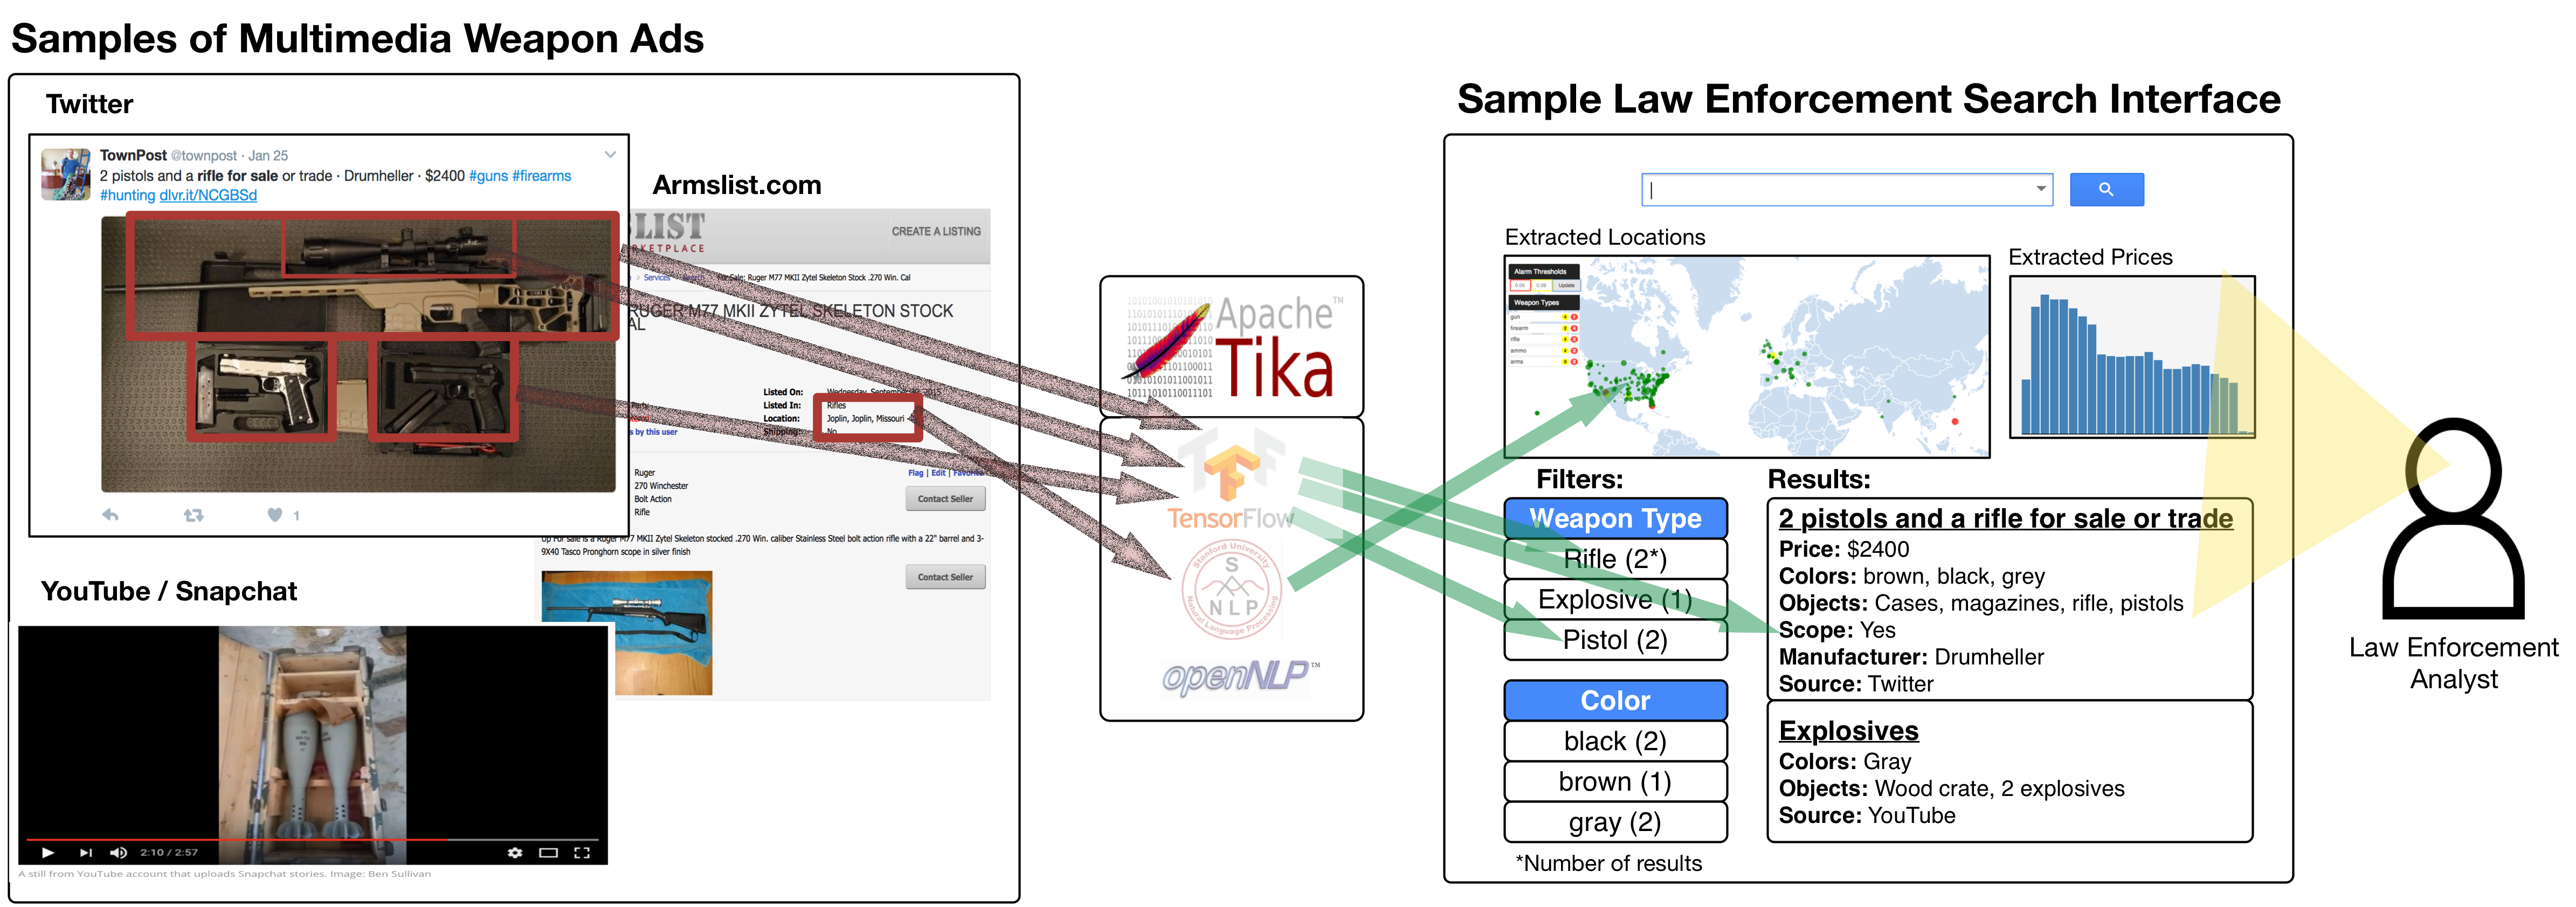
\includegraphics[width=\textwidth,height=6cm]{interface-diagram}
	\caption{This diagram demonstrates how the integration of Tika and Tensorflow facilitates in-depth search across heterogenuous content types. There are several extensions to our object recognition implementation as well, including more refined categories, optical-character recognition, and image similarity metrics.}
	\label{fig:interface-diagram}
\end{figure*}

\section{Data Collection and Content Analysis in Memex}
\label{sec:memex-data}
% This section discusses motivations behind DARPA Memex and provides background on program data. 
Current commercial search engines provide generalized search interfaces that allow users to search across a limited portion of the web~\cite{}. However, in the context of cyber security and law enforcement, commercial search engines miss essential content from the Deep and Dark Web. Because it is hard to reach, this content often harbors illicit activity. The goal of Memex is to develop softwares that can quickly and thoroughly collect, organize, and search subsets of information relevant to individual domains of interest. The initial program focus was centered on illegal weapons trade and human trafficking.

To start, several enhanced web crawlers were used to discover and retrieve information from the websites related to target domains. Along with the general-purpose web crawlers, specialized crawlers were used for the retrieval of Dark web data using The Onion Router (TOR) protocol \cite{mentor2016onion} and also specialized in the retrieval of dynamic AJAX content guarded by login forms. Fetched data were then cached within the system for analysis due to the ephemeral nature of the source (web) content.

% \subsection{Memex Dataset} \label{sec:memex-dataset}
The dataset used in our experiment was a subset of Memex dataset; it contained 7.2 million documents in the illegal weapon sales domain, of which 1.4 million documents were images. We analyzed the textual documents in a different experiment using named-entity recognition (NER) models that extracted people, locations, organizations, weapon names, and weapon-types. Tika has recently added support for this task using popular Natural Language Processing toolkits like Stanford CoreNLP\cite{Finkel:2005:INI:1219840.1219885}, Apache OpenNLP\cite{ApacheOpenNLP}, and MIT Lincoln Lab's MITIE \cite{MITIE-github}. In the experiment described here, we generated semantic labels for image-based objects by classifying them into various categories.

% \section{CONTENT ANALYSIS IN MEMEX PROGRAM} \label{sec:memex}
While a majority of web content consists of either plain or rich text \cite{mphillips-EOT2012}, resource-constrained law enforcement agencies are further challenged by the fact that important information is often embedded in rich content (images, audio, video) present in weapons ads. Generally,  the need for computer vision and pixel-based analysis has increased with the rise of multimedia. Consequently Tika now provides support for one of the most popular and well-documented deep learning frameworks, Google's Tensforflow. As menioned in Section 1, our initial integration of Tensorflow is focused around object recognition, which serves two primary purposes: web crawlers generally extract any linked content from a site and ensuring images contained relevant objects was an important preprocessing step, and classifying image objects allows for the cataloguing of specific objects of interest. 

% Object recognition is a standard problem in computer vision which deals with the recognition of objects of interest in the graphical data. In the context of images it is often called as image recognition. Historically image recognition was a challenging task and its accuracy of the recognized objects were much lower than average Human performance. However, due to the recent advancements in deep neural networks and availability of larger datasets with faster computing resources, we now have systems which have nearer or better performance than average human beings\cite{karpathy-cnn-compare}.

% Today's deep learning frameworks are focused towards performance gain from native code and GPU optimization for fast matrix manipulations. One of the most popular and well-documented deep-learning systems is Google's Tensorflow \cite{abadi2016tensorflow}. Tensorflow is a scalable, Python-based system and it natively supports image recognition via its {\em Inception} model \cite{abadi2016tensorflow}. Inception provides a neural network trained on the ImageNet corpus \cite{krizhevsky2012imagenet}, a dataset of 14,197,122 images and classified using the WordNet taxonomy. As such, Tensor 

\label{sec:memex-tools}
The ultimate goal of integrating and characterizing diverse content scattered across the web is to provide law enforcement analysts with tools that will help them quickly identify potentially illegal activity, and images and videos often provide salient information not available in text; in many cases, illegal weapons dealers intentionally embed revealing details in rich content mediums because they are harder to identify. This thinking coincides with the rise of weapons trafficking on social media platforms such as Snapchat, YouTube, and Instagram, where communication is centered around images and video \cite{socialmedia}. The integration of Tensorflow and Tika provides a single, streamlined platform that unites the extraction of textual and rich content. This combined content can then be exposed through search and visualization interfaces that improve analysts' abilities to drill-down and explore comprehensive, diverse content contained in weapons ads (see Figure \ref{fig:interface-diagram}). 